Užtriukšminti karo pabėgėlių ir žodžio „war“ skaičius per mėnesį signalai (~\ref{fig:noisy} pav.) gauti panaudojus paprastą atsitiktinių skaičių (random) generatorių \(y = x * rand\), kai \(rand\) generuoja reikšmes iš \((0, 1)\). Tada, pakeičiant švarų signalą užtriukšmintu, paskaičiuota signalų tarpusavio koreliacija.

\begin{figure}
    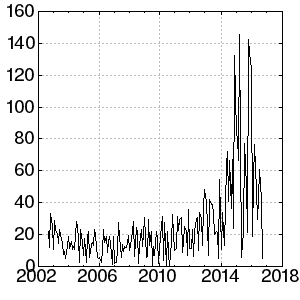
\includegraphics[scale=0.65]{../scripts/refugees_war_rand/refugees_rand.png}
    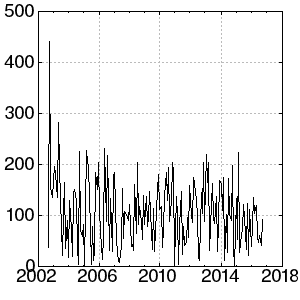
\includegraphics[scale=0.65]{../scripts/refugees_war_rand/war_rand.png}
    \caption{Grafikas kairėje: užtriukšmintas bendras mėnesinis karo pabėgėlių skaičius pasaulyje (tūkstančiais). Grafikas dešinėje: užtriukšmintas mėnesinis „war“ žodžio dažnumas ABC naujienų antraštėse.}
    \label{fig:noisy}
\end{figure}

\begin{figure}
    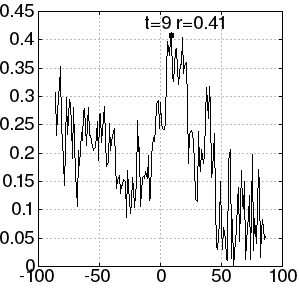
\includegraphics[scale=0.65]{../scripts/refugees_war_rand/result_ref_rand.png}
    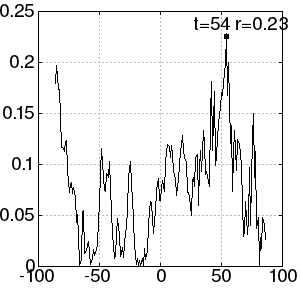
\includegraphics[scale=0.65]{../scripts/refugees_war_rand/result_war_rand.png}
    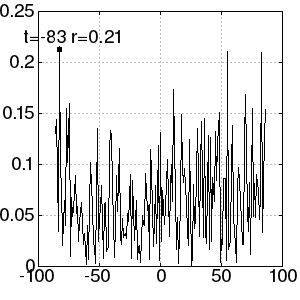
\includegraphics[scale=0.65]{../scripts/refugees_war_rand/result_both_rand.png}
    \caption{Grafikas kairėje: užtriukšminto pabėgėlių ir švaraus „war“ dažnumo koreliacija. Grafikas centre: švaraus pabėgėlių ir užtriukšminto „war“ dažnumo koreliacija. Grafikas dešinėje: signalų tarpusavio koreliacija kai abu signalai užtiukšminti.}
    \label{fig:noisy_cross}
\end{figure}

Iš koreliacijos grafikų (~\ref{fig:noisy_cross} pav. ) matosi, kad užtriukšmintas pabėgelių skaičius nestipriai pakeitė algoritmo rezultatus.
Bet tokiu pačiu metodu užtriukšmintas „war“ žožio dažnumas daug stipririau iškreipė koreliacijos grafiką, kai pabėgėlių signalas buvo švarus.
Užtriukšminus abu signalus, algoritmas neberanda vidutinės koreliacijos tarp jų ir grafike matosi atsiradę keletas naujų lokalių maksimumų.
